\chapter{Evaluation}
\label{chap:Evaluation}
\mtoc

In this chapter, we evaluate the method names generated by our model. We start by discussing the complexity of such an evaluation. Then we describe several metrics that we have selected for automatic evaluation, apply them to the generated names, and compare the scores of our model to several baseline models.

\section{Why is it hard to evaluate names?}
\label{sec:Evaluation-WhyHard}

While consistency of naming can be evaluated using simple heuristics that measure how much does a given name fit into the family of existing names, there is no objective way to tell how well does a given name represent certain concepts, usage, or implementation details. Human languages are complex and not formal. There can be many ways of describing the purpose of a method, class, or variable in 2-5 English words. And there can be many opinions on how comprehensive and informative a certain name is.

\subsection{Human evaluation}

Since our goal is to improve the readability of source code, the best way to evaluate the conciseness of identifier names would be asking a group of developers to evaluate them independently and then aggregating these results to produce a single score that would be most representative of human comprehension. The main drawback of human evaluation is its high cost in terms of human-hours and very low speed of evaluation. This means that we can only evaluate a reasonably small subset of methods using human experts and can only conduct this evaluation once or twice.

\subsection{Automatic evaluation}

Automatic metrics such as precision can be calculated quickly and do not require any additional expenses or involvement of human experts. The disadvantage of those metrics is the fact that they are very simplified approximate measures of goodness and informativeness of method names which nevertheless are very useful in practice.

Automatic metrics can only compare generated names to a set of reference names provided by humans that are considered to be a golden standard. More specifically, precision can measure the percentage of words in a generated method name that also appear in the real name of that method. When averaged over a big dataset of methods, precision can be very useful for comparing two different models. However, it can not be reliably used for evaluating a single name or interpreted as a standalone measure of model's performant because everything that is different from a reference name will be given a score of $0$. Automatic metrics are very simple measures that cannot recognize synonyms or different grammatical forms of words.

For example, if the real method name is \texttt{sumOfIntegers}, a reasonably good name such as \texttt{addAllIntegerNumbers} will be scored with 0 by all metrics discussed in the following section, because none of the words in those names match exactly. However, as we have seen in section \ref{sec:Naturalness-Vocabulary}, vocabulary used by programmers is very limited. Synonyms and different word forms are rather rare in practice, which means that in real-world scenarios automatic metrics can provide a pretty good approximation of the true model performance.

\section{Automatic evaluation}

As we said before, all metrics for automatic evaluation of method names are based on comparing the \textbf{generated name} to one or more \textbf{reference names} that are given by humans and considered the ground truth. Since all methods in our study were collected from real projects, each of them has exactly one name associated with it that was given by a programmer.

\subsection{Hypothesis for automatic evaluation}

As it was explained in Section \ref{sec:Evaluation-WhyHard}, automatic metrics are very simplified and imperfect. However, we can use them to compare different models based on the hypothesis that on average better model will generate more names similar to the real names of the methods.

\begin{quote}
Given a set of method bodies and a set of real method names, on average the names generated by a good model will be more similar to real names than the names from a bad model.
\end{quote}

It is important to keep this assumption in mind when looking at the results of the automatic evaluation and remember that it only holds when averaging multiple scores. On the level of individual observations, a method name with low precision score can be more relevant and informative than the name with a higher score.

\subsection{Selecting metrics}
\label{sec:Evaluation-Metrics}

In this section, we define the metrics that we have used for the automatic evaluation of method names generated by our model. We explain how each one of them works and provide examples of method names together with scores assigned to them by the metric in question. The method names in our examples were selected to demonstrate differences between those metrics:

\begin{description}
  \item [\texttt{testIsInteger}] \hfill \\
      --- exactly matches the reference name
  \item [\texttt{isIntegerTest}] \hfill \\
      --- has all the same words as the reference name but in different order
  \item [\texttt{testInteger}] \hfill \\
      --- has 2 out of 3 words of the reference name
  \item [\texttt{testIntegerNumber}] \hfill \\
      --- has 2 out of 3 words of the reference name and one additional word
  \item [\texttt{testIsIntegerNumber}] \hfill \\
      --- has all words of the reference name and one additional word
\end{description}

\paragraph{Exact match} --- percentage of generated method names that match reference names exactly (including the order of words). This metric was inspired by \cite{Alla16}.

\begin{table}[H]
\centering
\begin{tabular}{|l|r|}
  \hline
  testIsInteger & 1.00 \\
  \hline
  isIntegerTest & 0.00 \\
  \hline
  testInteger & 0.00 \\
  \hline
  testIsNumber & 0.00 \\
  \hline
  testIsIntegerNumber & 0.00 \\
  \hline
\end{tabular}
\caption{Exact match scores of names generated for a method with real name testIsInteger}
\end{table}

\paragraph{Precision} --- percentage of words in the generated name that appear in a reference name. It is calculated as a fraction of true positives ($\TP$\footnote{We use the following notation: $\TP$ - number of true positives, $\FP$ - number of false positives, $\TN$ - number of true negatives, $\FN$ - number of false negatives}) - number of words that appear both in reference and the generated name, by the total number of words in a generated name ($\TP + \FP$).

\[
\precision = \frac{\TP}{\TP + \FP}
\]

\begin{table}[H]
\centering
\begin{tabular}{|l|r|}
  \hline
  testIsInteger & 1.00 \\
  \hline
  isIntegerTest & 1.00 \\
  \hline
  testInteger & 1.00 \\
  \hline
  testIsNumber & 0.67 \\
  \hline
  testIsIntegerNumber & 0.75 \\
  \hline
\end{tabular}
\caption{Precision scores of names generated for a method with real name testIsInteger}
\end{table}

\paragraph{Recall} --- percentage of words in the reference name that appear in a generated name. It is calculated as a fraction of true positives ($\TP$) - the number of words that appear both in reference and the generated name, by the total number of words in a reference name ($\TP + \FN$).

\[
\recall = \frac{\TP}{\TP + \FN}
\]

\begin{table}[H]
\centering
\begin{tabular}{|l|r|}
  \hline
  testIsInteger & 1.00 \\
  \hline
  isIntegerTest & 1.00 \\
  \hline
  testInteger & 0.67 \\
  \hline
  testIsNumber & 0.67 \\
  \hline
  testIsIntegerNumber & 1.00 \\
  \hline
\end{tabular}
\caption{Recall scores of names generated for a method with real name testIsInteger}
\end{table}

\paragraph{F1} --- harmonic mean\footnote{Harmonic mean is more intuitive than the arithmetic mean when computing a mean of ratios} of precision and recall (\cite{Sasa07}).

\[
\fone = 2 \cdot \frac{\precision \cdot \recall}{\precision + \recall}
\]

\begin{table}[H]
\centering
\begin{tabular}{|l|r|}
  \hline
  testIsInteger & 1.00 \\
  \hline
  isIntegerTest & 1.00 \\
  \hline
  testInteger & 0.80 \\
  \hline
  testIsNumber & 0.67 \\
  \hline
  testIsIntegerNumber & 0.86 \\
  \hline
\end{tabular}
\caption{$\fone$ scores of names generated for a method with real name testIsInteger}
\end{table}

% \subsubsection{BLEU}
%
% Bilingual evaluation understudy (\bleu), introduced by \cite{Papi02}, is the most commonly used metric for automatically evaluating machine translation.

\subsection{Baseline models for comparison}
\label{sec:Evaluation-Baselines}

To evaluate the performance of our model using automatic metrics described in Section \ref{sec:Evaluation-Metrics} we compare them to several simple baseline models applied to the same dataset.

\subsubsection{Random model}

When evaluating machine learning models, it is always important to understand what would the values of all selected metrics be if the model did not learn anything but only made random choices. For example, in the problem of handwritten digit recognition on a well-balanced dataset\footnote{Take MNIST dataset for example: \url{http://yann.lecun.com/exdb/mnist/}} 10\% accuracy can be achieved by randomly selecting one of the 10 digits. If the trained model has significantly more than 10\% accuracy, we can say that it has recognized some patterns in the data and learned to use them.

Our random model makes assumption that all words in vocabulary are uniformly distributed (equally likely to appear at any position in a name of any method) and generates names for test set methods by selecting $K$ random words from the training set vocabulary (vocabulary from which the words are selected is the output vocabulary described in Section \ref{sec:TranslatingCode-EncodingTokens} that was constructed from method names in the training set). In our case, $K=3$ is the average number of tokens in the method names from our dataset. We do not use the test set vocabulary because it can have words that are not present in the training set. This simulates the real-world situation as we can not know in advance the complete vocabulary that people will use for naming new methods to which our model will be applied.

\subsubsection{TF-IDF model}

\textit{Term Frequency - Inverse Document Frequency} (TF-IDF) is a measure of word importance. It works by determining the relative frequency of a word in a specific method compared to the inverse proportion of that word over the entire corpus of source code. Intuitively, this calculation determines how relevant a given word is in a particular method (\cite{Ramo03}). Words that is rare in the entire source code corpus, but appears a lot in the code of a particular method must be strongly related to the concepts that describe the purpose of that method. Words that are common in all methods such as \texttt{self}, \texttt{if}, \texttt{true} receive low TF-IDF scores and are not selected into the method name.

Despite its simplicity and the fact that it generates method names using the source code vocabulary, TF-IDF algorithm achieves surprisingly good results in terms of automatic metrics described in Section \ref{sec:Evaluation-Metrics}. This is a simple and effective statistical technique that can be used as a good baseline to compare our model to.

TF-IDF score of a word $w$ in method $m$ that is part of a source code corpus $C$ is computed as a product of its \textit{term frequency} (TF) and \textit{inverse document frequency} (IDF).

\[ \tfidf(w, m, C) = \tf(w, m) \cdot \idf(w, C) \]

Where term frequency is defined as $f_{w,m}$ - number of times word $w$ appears in the source code of method $m$.

\[ \tf(w, m) = f_{w,m} \]

And inverse document frequency is the logarithm of $|C|$ - total number of words in source code corpus $C$ divided by $f_{w,C}$ - the number of methods in $C$ in which the word $w$ appears.

\[ \idf(w, C) = \log \frac{|C|}{f_{w,C}} \]

Multiplying term frequency of a word by its inverse document frequency we penalize words that frequently occur in the language (see Section \ref{sec:Naturalness-SpecializedVocabulary}) and select only those that are frequent in a given context\footnote{In Section \ref{sec:Conclusion-TFIDF} where we describe a potential direction of future work you can find an interesting example of how TF-IDF can be used to group packages by their conceptual similarity.}. The algorithm computes TF-IDF scores for every token in the source code of a method and selects $K=3$ words with the highest score into the name.


\subsection{Results of automatic evaluation}

In this section, we present the numeric results of the automatic evaluation and use it to compare the performance of our model to the selected baseline models described in Section \ref{sec:Evaluation-Baselines}.

In Section \ref{sec:TranslatingCode-TrainValidTest} we have talked about splitting our dataset into three subsets for training, validation, and testing. The small size of the validation set and the fact that automatic metrics described in Section \ref{sec:Evaluation-Metrics} can be computed very quickly allowed us to perform an evaluation of our model every 1000 iterations of its training. On Figure \ref{fig:ValidScores} you can see how the performance of the model measured by different metrics improves during training and how it surpasses the TF-IDF baseline applied to the same methods from the validation subset. The random model baseline cannot be seen on this graph because all its scores are very close to 0.

\begin{figure}[H]
    \centering
    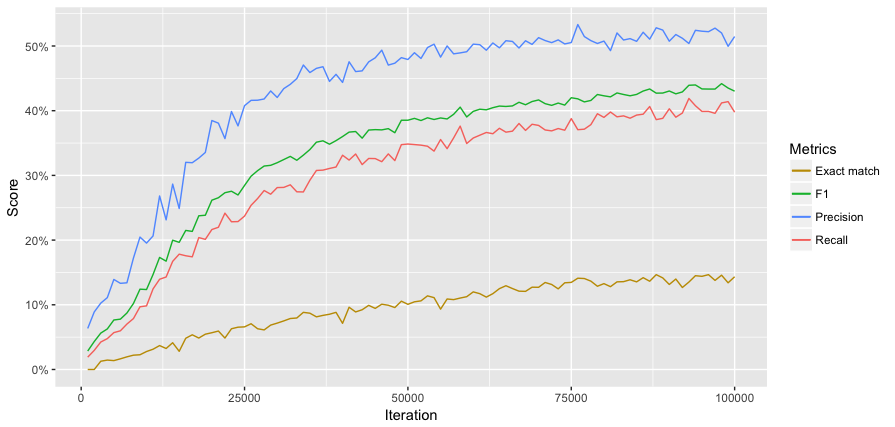
\includegraphics[width=\linewidth]{valid_scores}
  \caption{Evaluation of our model during training. Every 1000 iterations we applied the model to the validation set and measured all scores. Every score is compared to the corresponding value of the TF-IDF baseline (dashed lines)}
  \label{fig:ValidScores}
\end{figure}

Finally, we report the scores of our model together with baseline models measured on an independent test set which was never seen neither by model during training nor by us during model selection.

\begin{table}[H]
\centering
\begin{tabular}{|l|r|r|r|r|r|r|}
  \hline
  & Exact match & Precision & Recall & F1 \\
  \hline
  Our model & 13.82\% & 51.09\% & 38.92\% & 42.47\% \\
  \hline
  TF-IDF & 0.32\% & 28.61\% & 38.54\% & 30.95\% \\
  \hline
  Random model & 0\% & 0.07\% & 0.08\% & 0.07\% \\
  \hline
\end{tabular}
\caption{Results of automatic evaluation of method names generated by the selected models for methods from the test set}
\label{tab:Evaluation-TestResults}
\end{table}

In Table \ref{tab:Evaluation-TestResults} you can see the numeric scores of our model compared to selected baselines on the test set. First of all, notice that the random model has all scores close to 0. Both our model and TF-IDF perform significantly better, which proves that they indeed extract a lot of information from source code and successfully learn to generate method names. Our attention-based sequence to sequence deep neural network outperforms TF-IDF in terms of all metrics. By choosing parameters that maximize the likelihood of method names from our training set (see Section \ref{sec:TranslatingCode-Problem} and \ref{sec:Background-Likelihood}) our model guesses over 50\% of tokens from the previously unseen test set names.

Exact match is an interesting score because it demonstrates the ability of the model to not only to select frequent and relevant words but also put them in the correct order. Despite the fact that method name can be any combination of words from the vocabulary, which gives us really big space of possible names (and explains 0\% of exact match achieved by random model), our model guesses almost 14\% of names exactly. One can suspect that those are single word names. However, as you can see in Table \ref{tab:Evaluation-ExactMatches},  most of the exactly matched names have more than one word and some of them are novel names that have never appeared in the training set.

\begin{table}[H]
\centering
\begin{tabular}{|l|r|r|r|r|}
  \hline
  \textbf{Length} & \textbf{Unique names} & \textbf{\% of test set} & \textbf{Appear in train set} & \textbf{Novel names} \\
  \hline
  1 word & 249 & 6.63\% & 245 & 4 \\
  \hline
  2 words & 351 & 5.80\% & 301 & 50 \\
  \hline
  3 words & 108 & 1.09\% & 75 & 33 \\
  \hline
  4 words & 16 & 0.19\% & 11 & 5 \\
  \hline
  5 words & 10 & 0.09\% & 10 & 0 \\
  \hline
  6 words & 1 & 0.01\% & 1 & 0 \\
  \hline
  8 words & 1 & 0.01\% & 1 & 0 \\
  \hline
\end{tabular}
\caption{Distribution of names generated by our model that match real method names exactly over the length of the name (number of sub-token words). Columns of this table show the number of unique names in each group, what percent of all names from training set are in the group, how many of those names appeared in training set (but were paired with different source code), and how many names were never seen by the model before}
\label{tab:Evaluation-ExactMatches}
\end{table}

It is worth noting that despite its simplicity, TF-IDF performs reasonably well. Deep models are expensive both in terms of training and the complexity of deployment: big memory consumption by a trained model, high overhead when producing a single result. So in those cases when deep learning may be inapplicable, a simpler statistical model such as TF-IDF can be combined with other algorithms (for example, n-gram model for ordering words or hand-written heuristics) to produce very good results.

% \section{Human evaluation}
%
% \subsection{Design of questionnaire}
%
% \subsection{Results of evaluation}
